\documentclass[12pt,a4paper]{article}
	%[fleqn] %%% --to make all equation left-algned--

% \usepackage[utf8]{inputenc}
% \DeclareUnicodeCharacter{1D12A}{\doublesharp}
% \DeclareUnicodeCharacter{2693}{\anchor}
% \usepackage{dingbat}
% \DeclareRobustCommand\dash\unskip\nobreak\thinspace{\textemdash\allowbreak\thinspace\ignorespaces}
\usepackage[top=2in, bottom=1in, left=1in, right=1in]{geometry}
%\usepackage{fullpage}

\usepackage{fancyhdr}\pagestyle{fancy}\rhead{Stephanie Wang}\lhead{EE236B homework 3}

\usepackage{amsmath,amssymb,amsthm,amsfonts,microtype,stmaryrd}
	%{mathtools,wasysym,yhmath}

\usepackage[usenames,dvipsnames]{xcolor}
\newcommand{\blue}[1]{\textcolor{blue}{#1}}
\newcommand{\red}[1]{\textcolor{red}{#1}}
\newcommand{\gray}[1]{\textcolor{gray}{#1}}
\newcommand{\fgreen}[1]{\textcolor{ForestGreen}{#1}}

\usepackage{mdframed}
	%\newtheorem{mdexample}{Example}
	\definecolor{warmgreen}{rgb}{0.8,0.9,0.85}
	% --Example:
	% \begin{center}
	% \begin{minipage}{0.7\textwidth}
	% \begin{mdframed}[backgroundcolor=warmgreen, 
	% skipabove=4pt,skipbelow=4pt,hidealllines=true, 
	% topline=false,leftline=false,middlelinewidth=10pt, 
	% roundcorner=10pt] 
	%%%% --CONTENTS-- %%%%
	% \end{mdframed}\end{minipage}\end{center}	

\usepackage{graphicx} \graphicspath{{}}
	% --Example:
	% \includegraphics[scale=0.5]{picture name}
%\usepackage{caption} %%% --some awful package to make caption...

\usepackage{hyperref}\hypersetup{linktocpage,colorlinks}\hypersetup{citecolor=black,filecolor=black,linkcolor=black,urlcolor=blue,breaklinks=true}

%%% --Text Fonts
%\usepackage{times} %%% --Times New Roman for LaTeX
%\usepackage{fontspec}\setmainfont{Times New Roman} %%% --Times New Roman; XeLaTeX only

%%% --Math Fonts
\renewcommand{\v}[1]{\ifmmode\mathbf{#1}\fi}
%\renewcommand{\mbf}[1]{\mathbf{#1}} %%% --vector
%\newcommand{\ca}[1]{\mathcal{#1}} %%% --"bigO"
%\newcommand{\bb}[1]{\mathbb{#1}} %%% --"Natural, Real numbers"
%\newcommand{\rom}[1]{\romannumeral{#1}} %%% --Roman numbers

%%% --Quick Arrows
\newcommand{\ra}[1]{\ifnum #1=1\rightarrow\fi\ifnum #1=2\Rightarrow\fi\ifnum #1=3\Rrightarrow\fi\ifnum #1=4\rightrightarrows\fi\ifnum #1=5\rightleftarrows\fi\ifnum #1=6\mapsto\fi\ifnum #1=7\iffalse\fi\fi\ifnum #1=8\twoheadrightarrow\fi\ifnum #1=9\rightharpoonup\fi\ifnum #1=0\rightharpoondown\fi}

%\newcommand{\la}[1]{\ifnum #1=1\leftarrow\fi\ifnum #1=2\Leftarrow\fi\ifnum #1=3\Lleftarrow\fi\ifnum #1=4\leftleftarrows\fi\ifnum #1=5\rightleftarrows\fi\ifnum #1=6\mapsfrom\ifnum #1=7\iffalse\fi\fi\ifnum #1=8\twoheadleftarrow\fi\ifnum #1=9\leftharpoonup\fi\ifnum #1=0\leftharpoondown\fi}

%\newcommand{\ua}[1]{\ifnum #1=1\uparrow\fi\ifnum #1=2\Uparrow\fi}
%\newcommand{\da}[1]{\ifnum #1=1\downarrow\fi\ifnum #1=2\Downarrow\fi}

%%% --Special Editor Config
\renewcommand{\ni}{\noindent}
\newcommand{\onum}[1]{\raisebox{.5pt}{\textcircled{\raisebox{-1pt} {#1}}}}

\newcommand{\claim}[1]{\underline{``{#1}":}}

\renewcommand{\l}{\left}\renewcommand{\r}{\right}

\newcommand{\casebrak}[2]{\left \{ \begin{array}{l} {#1}\\{#2} \end{array} \right.}
%\newcommand{\ttm}[4]{\l[\begin{array}{cc}{#1}&{#2}\\{#3}&{#4}\end{array}\r]} %two-by-two-matrix
%\newcommand{\tv}[2]{\l[\begin{array}{c}{#1}\\{#2}\end{array}\r]}

\def\dps{\displaystyle}

\let\italiccorrection=\/
\def\/{\ifmmode\expandafter\frac\else\italiccorrection\fi}


%%% --General Math Symbols
\def\bc{\because}
\def\tf{\therefore}

%%% --Frequently used OPERATORS shorthand
\newcommand{\INT}[2]{\int_{#1}^{#2}}
% \newcommand{\UPINT}{\bar\int}
% \newcommand{\UPINTRd}{\overline{\int_{\bb R ^d}}}
\newcommand{\SUM}[2]{\sum\limits_{#1}^{#2}}
\newcommand{\PROD}[2]{\prod\limits_{#1}^{#2}}
\newcommand{\CUP}[2]{\bigcup\limits_{#1}^{#2}}
\newcommand{\CAP}[2]{\bigcap\limits_{#1}^{#2}}
% \newcommand{\SUP}[1]{\sup\limits_{#1}}
% \newcommand{\INF}[1]{\inf\limits_{#1}}
\DeclareMathOperator*{\argmin}{arg\,min}
\DeclareMathOperator*{\argmax}{arg\,max}
\newcommand{\pd}[2]{\frac{\partial{#1}}{\partial{#2}}}
\def\tr{\text{tr}}

\renewcommand{\o}{\circ}
\newcommand{\x}{\times}
\newcommand{\ox}{\otimes}

\newcommand\ie{{\it i.e. }}
\newcommand\wrt{{w.r.t. }}
\newcommand\dom{\mathbf{dom\:}}

%%% --Frequently used VARIABLES shorthand
\def\R{\ifmmode\mathbb R\fi}
\def\N{\ifmmode\mathbb N\fi}
\renewcommand{\O}{\mathcal{O}}

\newcommand{\dt}{\Delta t}
\def\vA{\mathbf{A}}
\def\vB{\mathbf{B}}\def\cB{\mathcal{B}}
\def\vC{\mathbf{C}}
\def\vD{\mathbf{D}}
\def\vE{\mathbf{E}}
\def\vF{\mathbf{F}}\def\tvF{\tilde{\mathbf{F}}}
\def\vG{\mathbf{G}}
\def\vH{\mathbf{H}}
\def\vI{\mathbf{I}}\def\cI{\mathcal{I}}
\def\vJ{\mathbf{J}}
\def\vK{\mathbf{K}}
\def\vL{\mathbf{L}}\def\cL{\mathcal{L}}
\def\vM{\mathbf{M}}
\def\vN{\mathbf{N}}\def\cN{\mathcal{N}}
\def\vO{\mathbf{O}}
\def\vP{\mathbf{P}}
\def\vQ{\mathbf{Q}}
\def\vR{\mathbf{R}}
\def\vS{\mathbf{S}}
\def\vT{\mathbf{T}}
\def\vU{\mathbf{U}}
\def\vV{\mathbf{V}}
\def\vW{\mathbf{W}}
\def\vX{\mathbf{X}}
\def\vY{\mathbf{Y}}
\def\vZ{\mathbf{Z}}

\def\va{\mathbf{a}}
\def\vb{\mathbf{b}}
\def\vc{\mathbf{c}}
\def\vd{\mathbf{d}}
\def\ve{\mathbf{e}}
\def\vf{\mathbf{f}}
\def\vg{\mathbf{g}}
\def\vh{\mathbf{h}}
\def\vi{\mathbf{i}}
\def\vj{\mathbf{j}}
\def\vk{\mathbf{k}}
\def\vl{\mathbf{l}}
\def\vm{\mathbf{m}}
\def\vn{\mathbf{n}}
\def\vo{\mathbf{o}}
\def\vp{\mathbf{p}}
\def\vq{\mathbf{q}}
\def\vr{\mathbf{r}}
\def\vs{\mathbf{s}}
\def\vt{\mathbf{t}}
\def\vu{\mathbf{u}}
\def\vv{\mathbf{v}}\def\tvv{\tilde{\mathbf{v}}}
\def\vw{\mathbf{w}}
\def\vx{\mathbf{x}}\def\tvx{\tilde{\mathbf{x}}}
\def\vy{\mathbf{y}}
\def\vz{\mathbf{z}}

%%% --Numerical analysis related
%\newcommand{\nxt}{^{n+1}}
%\newcommand{\pvs}{^{n-1}}
%\newcommand{\hfnxt}{^{n+\frac12}}

%%%%%%%%%%%%%%%%%%%%%%%%%%%%%%%%%%%%%%%%%%%%%%%%%%%%%%%%%%%%%%%%%%%%%%%%%%%%%%%%%%%%%%%%%%%%%%%%%%%%%%%%%%%%%%%%%%%%%%%%%%%%%%%%%%%%%%%%%%%%%%%%%%%%%%%%%%%%%%%%%%%%%%%%%%%%%%%%%%%%%%%%%%%%%%%%%%%%%%
\begin{document}
\subsubsection*{Exercise 3.18 [Boyd \& Vandenberghe, 2004]}
\noindent Adapt the proof of concavity of the log-determinant function in \S 3.1.5 to show the following. \\
(a) $f(X) = \tr(X^{-1})$ is convex on $\dom f = \vS^n_{++}$.\\
(b) $f(X) = (\det X)^{1/n}$ is concave on $\dom f = \vS^n_{++}$.\\
\\
{\it Ans:} Here only does part (a).  \\
(a) It suffices to show $g(t) = \tr((X+tZ)^{-1})$ is convex \wrt $t\in [t_0,t_1]$ where $X \in \vS^n_{++}$, $Z \in \vS^n$ and $[t_0, t_1]$ is an interval such that $X+tZ$ remains positive definite. Use this \href{http://math.stackexchange.com/questions/478998/a-property-of-positive-definite-matrices}{property of positive definite matrix}, write 
$$X = S^{-1}S^{-T}, Z = S^{-1} L S^{-T}$$
then
\begin{align*}
g(t) &= \tr((X+tZ)^{-1})\\
&= \tr((S^{-1}(I+tL)S^{-T})^{-1})\\
&= \tr(S (I+tL)^{-1} S^T)\\
&= \tr(S^TS(I+tL)^{-1})\\
g'(t) &= \tr\l(S^TS\/{d}{dt} (I+tL)^{-1}\r) \\
&= -\tr(S^TS(I+tL)^{-1}L(I+tL)^{-1})
\end{align*}
Here I made use of the identity 
\begin{align*}
I & = A^{-1}(t)A(t)\\
O &= \l(\frac d{dt}A^{-1}(t)\r) A(t) + A^{-1}(t) A'(t) \\
\frac d{dt}A^{-1}(t) &= -A^{-1}(t) A'(t) A^{-1}(t)
\end{align*}
Now that $I+tL$ and $L$ are both diagonal, they commute. 
\begin{align*}
g'(t) &= -\tr(S^TS(I+tL)^{-1}L(I+tL)^{-1})\\
&= -\tr(S^TS L(I+tL)^{-2}) \\
g''(t) &= \tr(S^TSL ((I+tL)^{-2}L(I+tL)^{-1} + (I+tL)^{-1}L (I+tL)^{-2})) \\
&= 2\tr(SL^2 (I+tL)^{-3}S^T)
\end{align*}
Since $t$ is such that $X+tZ = S^{-1} (I+tL) S^{-T} \succ 0$, $I+tL$ must be positive diagonal matrix, and $(I+tL)^{-3} \succ 0$; alongside with $L^2 \succeq 0$, we see $L^2(I+tL)^{-3} \succeq 0$, therefore
$$S L^2 (I+tL)^{-3} S^T \succeq 0$$
and $g''(t) \geq 0$ (\ie $g$ is convex). \qed



\newpage\subsubsection*{Exercise 3.19 [Boyd \& Vandenberghe, 2004]}
\noindent {\it Nonnegative weighted sums and integrals.} \\
(a) Show that $f(x) = \sum^r_{i=1}\alpha_ix_{[i]}$ is a convex function of $x$, where $\alpha_1 \geq \alpha_2 \geq \cdots \geq \alpha_r \geq 0$, and $x_{[i]}$ denotes the $i$th largest component of $x$. (You can use the fact that $f(x) = \sum_{i=1}^k x_{[i]}$ is convex on $\R^n$. )\\
(b) Let $T(x, \omega)$ denote the trigonometric polynomial
$$T(x,\omega) = x_1 + x_2 \cos\omega + x_3\cos2\omega + \cdots + x_n\cos(n-1)\omega.$$
Show that the function
$$f(x) = -\INT0{2x} \log T(x,\omega)d\omega$$
is convex on $\{x \in \R^n \mid T(x,\omega)>0, 0\leq \omega \leq 2\pi\}$. \\
\\
{\it Ans:} Here only does part (a). \\
(a) Let $\beta_i = \alpha_i - \alpha_{i+1}$; then observe
\begin{align*}
f(x) & = \SUM{i=1}r \alpha_i x_{[i]} \\
&= \alpha_r\SUM{i=1}rx_{[i]} + (\alpha_{r-1}-\alpha_r)\SUM{i=1}{r-1}x_{[i]} + \cdots + (\alpha_1 - \alpha_2)\SUM{i=1}1 x_{[i]} \\
&= \alpha_r \SUM{i=1}r x_{[i]} + \beta_{r-1}\SUM{i=1}{r-1}x_{[i]} + \cdots + \beta_1\SUM{i=1}{1}x_{[i]}
\end{align*}
is a linear combination of convex functions with nonnegative coefficients and therefore convex.  \qed


\newpage\subsubsection*{Exercise 3.22 [Boyd \& Vandenberghe, 2004]}
\noindent {\it Composition rules.} Show that the following functions are convex. \\
(a) $f(x) = -\log(-\log(\sum^m_{i=1} e^{a_i^T x + b_i}))$ on $\dom f = \{x \mid \sum^m_{i=1} e^{a_i^T x + b_i} < 1\}$. You can use the fact that $\log(\sum^n_{i=1} e^{y_i})$ is convex.\\
(b) $f(x, u, v) = -\sqrt{uv-x^Tx}$ on $\dom f = \{(x,u,v) \mid uv>x^T x, u, v>0\}$. Use the fact that $x^T x/u$ is convex in $(x, u)$ for $u>0$, and that $-\sqrt{x_1x_2}$ is convex on $\R^2_{++}$. \\
(c) $f(x,u,v) = -\log(uv-x^Tx)$ on $\dom f = \{(x,u,v) \mid uv>x^Tx, u,v>0\}$.\\
(d) $f(x,t) = -(t^p - \|x\|_p^p)^{1/p}$ where $p>1$ and $\dom f = \{(x, t) \mid t\geq \|x\|_p\}$. You can use the fact that $\|x\|^p_p/u^{p-1}$ is convex in $(x,u)$ for $u>0$ (see exercise 3.23), and that $-x^{1/p}y^{1-1/p}$ is convex on $\R^2_+$ (see exercise 3.16). \\
(e) $f(x,t) = -\log(t^p - \|x\|_p^p)$ where $p>1$ and $\dom f = \{(x,t) \mid t>\|x\|_p\}$. You can use the fact that $\|x\|^p_p/u^{p-1}$ is convex in $(x,u)$ for $u>0$ (see exercise 3.23).\\
\\
{\it Ans:} Here only does part (c).  \\
(c) Let $g(x,u,v) = uv-x^Tx$, then $\nabla g(x,u,v) = [-2x^T, v,u]$ and 
$$H_g(x,u,v) = \l[\begin{array}{ccc}
-2I & & \\
& & 1 \\
& 1 & \end{array}\r]$$
and for any $(x,u,v)\in\dom f$, 
$$[x^T,u,v]\l[\begin{array}{ccc}
-2I & & \\
& & 1 \\
& 1 & \end{array}\r]\l[\begin{array}{c}
x\\
u\\
v\end{array}\r] = -2x^Tx + 2uv >0$$
That is, $g$ is convex on $\dom f$. Now that $h = -\log(\cdot)$ is convex and nonincreasing, we conclude $f = -\log(g(\cdot))$ is convex on $\dom f$ as well. \qed


\newpage\subsubsection*{Additional Exercise 2.5 [Boyd \& Vandenberghe, 2017]}
\noindent {\it A perspective composition rule} [Mar\`echal]. Let $f:\R^n\ra1\R$ be a convex function with $f(0) \leq 0$.\\
(a) Show that the perspective $tf(x/t)$, with domain $\{(x,t)\mid t>0, x/t \in \dom f\}$, is nonincreasing as a function of $t$. \\
(b) Let $g$ be concave and positive on its domain. Show that the function
$$h(x) = g(x)f(x/g(x)), \;\;\; \dom h = \{x\in\dom g\mid x/g(x) \in \dom f\}$$
is convex. \\
(c) As an example, show that 
$$h(x) = \frac{x^Tx}{\l(\PROD{k=1}n x_k\r)^{1/n}}, \;\;\; \dom h = \R^n_{++}$$
is convex. \\
\\
{\it Ans:} Here only does part (a) and (b). \\
(a) Fix $x \in \R^n$, for any $0 < t_1 < t_2$ such that $x/t_1, x/t_2 \in \dom f$, note that 
$$\/{x}{t_2} = \/{t_1}{t_2} \/{x}{t_1} + \/{t_2-t_1}{t_2}\cdot 0$$
By convexity of $f$, 
\begin{align*}
f(x/t_2) & \leq \/{t_1}{t_2} f(x/t_1) + \l(1-\/{t_1}{t_2}\r) f(0) \\
t_2 f(x/t_2) - t_1 f(x/t_1) & \leq \l(1-\/{t_1}{t_2}\r) f(0) \leq 0
\end{align*}
we conclude that $t_2 f(x/t_2) \leq t_1 f(x/t_1)$, and $f$ is nonincreasing. \\
\\
(b) First I want to show for $\alpha, \beta \in [0,1]$ with $\alpha + \beta \leq 1$ and $x, y\in\dom f$, 
$$f(\alpha x + \beta y) \leq \alpha f(x) + \beta f(y)$$
Let $t = \alpha+\beta\leq 1$ and $\theta = \alpha/t$, then $1-\theta = \beta/t$. The original inequality now becomes
\begin{align*}
f(\theta tx + (1-\theta) ty) \leq \theta tf(x) + (1-\theta) tf(y)
\end{align*}
This can be proven since $f$ is convex and the perspective $h(t, x) = tf(x/t)$ is nonincreasing \wrt t, 
\begin{align*}
f(\theta tx + (1-\theta) ty) &\leq \theta f(tx) + (1-\theta)f(ty) \\
&= \theta h(1, tx) + (1-\theta) h(1, ty) \\
&\leq \theta h(t, tx) + (1-\theta) h(t, ty) \\
&= \theta tf(tx/t) + (1-\theta)tf(ty/t) = \theta tf(x) + (1-\theta)tf(y)
\end{align*}
Now for general $\theta \in [0, 1]$ and $x,y\in \dom h$, since $g$ is concave, 
$$\alpha = \/{\theta g(x)}{g(\theta x + (1-\theta)y)}, \beta = \/{(1-\theta)g(y)}{g(\theta x + (1-\theta)y)} \in [0, 1]$$ 
and $\alpha + \beta = \/{\theta g(x) + (1-\theta)g(y)}{g(\theta x + (1-\theta)y)}\leq 1$. Apply the above ``lemma", 
\begin{align*}
h(\theta x + (1-\theta)y) &= g(\theta x + (1-\theta)y) f\l(\frac{\theta x + (1-\theta)y}{g(\theta x + (1-\theta)y)}\r)\\
&=g(\theta x + (1-\theta)y) f\l(\/{\theta g(x)}{g(\theta x + (1-\theta)y)}\/{x}{g(x)} + \/{(1-\theta)g(y)}{g(\theta x + (1-\theta)y)}\/{y}{g(y)}\r)\\
&= g(\theta x + (1-\theta)y) f\l(\alpha\/{x}{g(x)} + \beta\/{y}{g(y)}\r)\\
&\leq g(\theta x + (1-\theta)y) \l(\alpha f\l(\/{x}{g(x)}\r) + \beta f\l(\/{y}{g(y)}\r)\r) \\
&= {\theta g(x)}f\l(\/{x}{g(x)}\r) + {(1-\theta)g(y)}f\l(\/{y}{g(y)}\r) \\
& = \theta h(x) + (1-\theta)h(y)
\end{align*}
(c) Consider $f(x) = x^T x$ and $g(x) = \l(\PROD{k=1}n x_k\r)^{1/n}$; they are both common convex functions. Then
\begin{align*}
h(x) & = g(x) f(x/g(x)) \\
&= \l(\PROD{k=1}n x_k\r)^{1/n} \/{x^Tx}{\l(\PROD{k=1}n x_k\r)^{2/n}}\\
& = \frac{x^Tx}{\l(\PROD{k=1}n x_k\r)^{1/n}}
\end{align*}
is convex, too, by part (b). \qed




\newpage\subsubsection*{Additional Exercise 2.30 [Boyd \& Vandenberghe, 2017]}
\noindent {\it Huber penalty.} The infimal convolution of two functions $f$ and $g$ on $\R^n$ is defined as 
$$h(x) = \inf_y (f(y) + g(x-y))$$
(see exercise 2.17). Show that the infimal convolution of $f(x) = \|x\|_1$ and $g(x) = (1/2) \|x\|^2_2$, \ie, the function 
$$h(x) = \inf_y (f(y) + g(x-y)) = \inf_y \l(\|y\|_1 + \/12\|x-y\|^2_2\r)$$
is the {\it Huber penalty}
$$h(x) = \SUM{i=1}n \phi(x_i), \;\;\; \phi(u) = \casebrak{u^2/2, |u|\leq 1}{|u|-1/2, |u|>1}$$
{\it Ans:} Observe first 
\begin{align*}
h(x) &= \inf_{y\in\R^n} \l(\SUM{i=1}n |y_i| + \/12 (x_i-y_i)^2\r) \\
&= \SUM{i=1}n \inf_{y_i} \l(|y_i| + \/12(x_i-y_i)^2\r)
\end{align*}
Let $g(x_i) = \inf_{y_i} |y_i| + \/12(x_i-y_i)^2$. In order to show $g(x_i) = \phi(x_i)$, observe first that for $x_i \geq 0$, the minimizing $y_i$ must also be nonnegative and vice versa. Consider the case $x_i \geq 0$, then
$$g(x_i) = \inf_{y} y + \/12(x_i - y)^2$$
And the minimizer $y$ satisfies 
$$\frac d{dy}\l( y + \/12(x_i - y)^2 \r) = 1 - (x_i-y) = 0$$
$$\frac {d^2}{dy^2}\l( y + \/12(x_i - y)^2 \r) = 1 > 0$$
therefore $\bar y = x_i - 1$. If $x_i \geq 1$ then the minimizer will be in the scope (we assumed we are minimizing among all $y\geq 0$) and 
$$g(x_i) = \bar y + \/12(x_i - \bar y)^2 = x_i - \/12$$
However, if $x_i < 1$, then $0$ would be a better minimizer and 
$$g(x_i) = 0 + \/12(x_i - 0)^2 = \/12 x_i^2$$
Concluding above, we have 
$$g(x_i) = \l\{\begin{array}{ll}
x_i-1/2& , 1\leq x_i\\ 
x_i^2/2&, 0<x_1<1
\end{array}\r.$$
Since the same should hold analogously for $x_i < 0$, we prove $g(x_i) = \phi(x_i)$ for $x_i$ in all ranges. \qed




\newpage\subsubsection*{Additional Exercise 2.31 [Boyd \& Vandenberghe, 2017]}
\noindent Suppose the function $h:\R\ra1\R$ is convex, nondecreasing, with $\dom h = \R$, and $h(t) = h(0)$ for $t\leq 0$. \\
(a) Show that the function $f(x) = h(\|x\|_2)$ is convex on $\R^n$.\\
(b) Show that the conjugate of $f$ is $f^\ast(y) = h^\ast(\|y\|_2)$.\\
(c) As an example, derive the conjugate of $f(x) = (1/p)\|x\|^p_2$ for $p>1$, by applying the result of part (b) with the function 
$$h(t) = \/1p \max \{0, t\}^p = \casebrak{\/1pt^p, t\geq 0}{0, t<0}$$
{\it Ans:} \\
(a) Let $g(x) = \|x\|_2$, then 
\begin{align*}
\nabla g(x) &= \/{x^T}{\|x\|_2} \\
H_g(x) &= \/{1}{\|x\|_2^2}\l(I\|x\|_2 - \/{x}{\|x\|_2}x^T\r) \\
&= \/{1}{\|x\|_2} \l(I - \/{1}{\|x\|_2^2}xx^T\r) \\
v^T H_g(x) v &= \/{1}{\|x\|_2}\l(\|v\|_2 - \/{(x^T v)^2}{\|x\|^2_2}\r) \geq 0 \mbox{ (by Cauchy inequality)}
\end{align*}
Since $h$ is convex and nondecreasing and $g = \|\cdot\|_2$ is convex, the composition $f = h\o g$ must be convex, too. \\
\\
(b) By definition,
\begin{align*}
f^\ast(y) &= \sup_{x\in \R^n} x^Ty - f(x)\\
&= \sup_{x\in\R^n} x^Ty-h(\|x\|_2) \\
&=  \max\l\{\sup_{x\neq 0} \|x\|_2 \l(\/{x}{\|x\|_2}\r)^Ty - h(\|x\|_2), -h(0)\r\}\\
&= \sup_{x\neq 0} \|x\|_2 \l(\/{x}{\|x\|_2}\r)^Ty  - h(\|x\|_2) \mbox{ \;\;\; (because $-h$ is nonincreasing)} \\
&= \sup_{x\neq 0} \|x\|_2 \|y\|_2 - h(\|x\|_2) \\
&= \sup_{t >0} t \|y\|_2 - h(t)
\end{align*}
The last equality follows from that the first term is maximized when $x$ is parallel to $y$. Now observe the definition of $h^\ast$
$$h^\ast(\|y\|_2) = \sup_{t\in \R} t\|y\|_2 - h(t)$$
This differs from $f^\ast(y)$ only by the range of the minimizing variable (it's $t>0$ for $f^\ast$ and $t\in \R$ for $h^\ast$); however, since $h(t) = h(0)$ for $t\leq 0$, that is, for any $t <  0$,
$$t\|y\|_2 - h(t) = t\|y\|_2 - h(0) \leq 0\cdot \|y\|_2 - h(0)$$
The minimizer for $h^\ast$ can't fall in $(-\infty, 0)$. Therefore we conclude $f^\ast(y) = h^\ast(\|y\|_2)$. \\
\\
(c) From the problem settings, $f(x) = \/1p \|x\|^p_2 = h(\|x\|_2)$. To show $f$ is convex, it suffices to show that $h$ is convex, nondecreasing and $h(t) = h(0)$ for $t\leq 0$. $h$ is convex since 
$$h'(t) = \casebrak{t^{p-1}, t\geq 0}{0, t<0}$$
is continuous and nondecreasing; $h$ is nondecreasing follows from $p>1$ and $h(t) = h(0)$ for $t\leq 0$ is just a part of the definition. \qed



\newpage\subsubsection*{Additional Exercise 3.17 [Boyd \& Vandenberghe, 2017]}
\noindent {\it Minimum fuel optimal control.} Solve the minimum fuel optimal control problem described in exercise 4.16 of {\it Convex Optimization}, for the instance with problem data
$$A = \l[\begin{array}{ccc}
-1&0.4&0.8\\
1&0&0\\
0&1&0\end{array}\r], b = \l[\begin{array}{c}
1\\
0\\
0.3\end{array}\r], x_{des} = \l[\begin{array}{c}
7\\
2\\
-6\end{array}\r], N = 30.$$
You can do this by forming the LP you found in your solution of exercise 4.16, or more directly using CVX. Plot the actuator signal $u(t)$ as a function of time $t$. 
\subsubsection*{Exercise 4.16 [Boyd \& Vandenberghe, 2004]}
{\it Minimum fuel optimal control.} We consider a linear dynamical system with state $x(t) \in \R^n$, $t = 0, \cdots, N$, and actuator or input signal $u(t) \in \R$, for $t=0, \cdots, N-1$. The dynamics of the system is given by the linear recurrence 
$$x(t+1) = Ax(t) + bu(t), t = 0, \cdots, N-1,$$
where $A \in \R^{n\x n}$ and $b\in \R^n$ are given. We assume that the initial state is zero, \ie, $x(0) = 0$. \\
The {\it minimum fuel optimal control problem} is to choose the inputs $u(0), \cdots, u(N-1)$ so as to minimize the total fuel consumed, which is given by
$$F = \SUM{i=0}{N-1} f(u(t)),$$
subject to the constraint that $x(N) = x_{des}$, where $N$ is the (given) time horizon, and $x_{des} \in \R^n$ is the (given) desired final or target state. The function $f:\R\ra1\R$ is the {\it fuel use map} for the actuator, and gives the amount of fuel used as a function of the actuator signal amplitude. In this problem we use 
$$f(a) = \l\{\begin{array}{cc}
|a| & |a|\leq 1\\
2|a|-1 & |a| > 1.\end{array}\r.$$
This means that fuel use is proportional to the absolute value of the actuator signal, for actuator signals between $-1$ and $1$; for larger actuator signals the marginal fuel efficiency is half. \\
Formulate the minimum fuel optimal control problem as an LP. \\
\\
{\it Ans:} 
The constraint is linear in $u(t)$, since $x(N)$ is a linear combination of $A^{N-1}b, \cdots, Ab, b$ with coefficients $u(0), \cdots, u(N-2), u(N-1)$,
\begin{align*} x(N) &= Ax(N-1) + bu(N-1)\\
&= A^2 x(N-2) + Abu(N-2) + bu(N-1)\\
&= \cdots \\
&= A^N x(0) + A^{N-1}bu(0) + A^{N-2}bu(1) + \cdots + Abu(N-2) + bu(N-1) \\
&=A^{N-1}bu(0) + A^{N-2}bu(1) + \cdots + Abu(N-2) + bu(N-1) 
\end{align*}
and the original constraint is not much but
$$x_{des} = A^{N-1}bu(0) + A^{N-2}bu(1) + \cdots + Abu(N-2) + bu(N-1) $$
On the other hand, by introducing new variable\footnote{credit to \href{http://www.math.ucla.edu/~minhrose/}{Minh Pham} for his great hint!} $y(t)$ with constraints
$$\pm u(t), \pm 2u(t)-1 \leq y(t)$$
we find 
\begin{align*}
f(u(t)) &= \casebrak{|u(t)|, |u(t)| \leq 1}{2|u(t)|-1, |u(t)|>1}\\
&= \max\{\pm u(t), \pm 2u(t)-1 \} \\
&= y(t)
\end{align*}
That is, the problem comes with $4*N + 3$ constraints on variables $u(t)$ and $y(t)$ with objective function $F = \SUM{i=0}{N-1} y(t)$. Or more formally speaking, the problem is 
$$\begin{array}{rl}
\mbox{minimize} & \mathbf{1}y\\
\mbox{subject to} & x_{des} = \mathcal K'(A,b)u\\
& u \leq y\\
& -u \leq y\\
& 2u-\mathbf{1} \leq y\\
& -2u - \mathbf{1} \leq y
\end{array}$$
where $\mathcal{K}'(A, b)$ is the Krylov matrix in reverse order
$$\mathcal K'(A, b) = \l[\begin{array}{cccc}
A^{N-1}b & \cdots & Ab & b
\end{array}\r]$$
Here's the graph of $u(t)$ as a function of $t$ and the codes used to generate the solution. I implemented the direct problem using CVX (plotted as blue line) as well as the linear programming problem (plotted as magenta crosses); it's encouraging that they give the same solution! 
\begin{center}
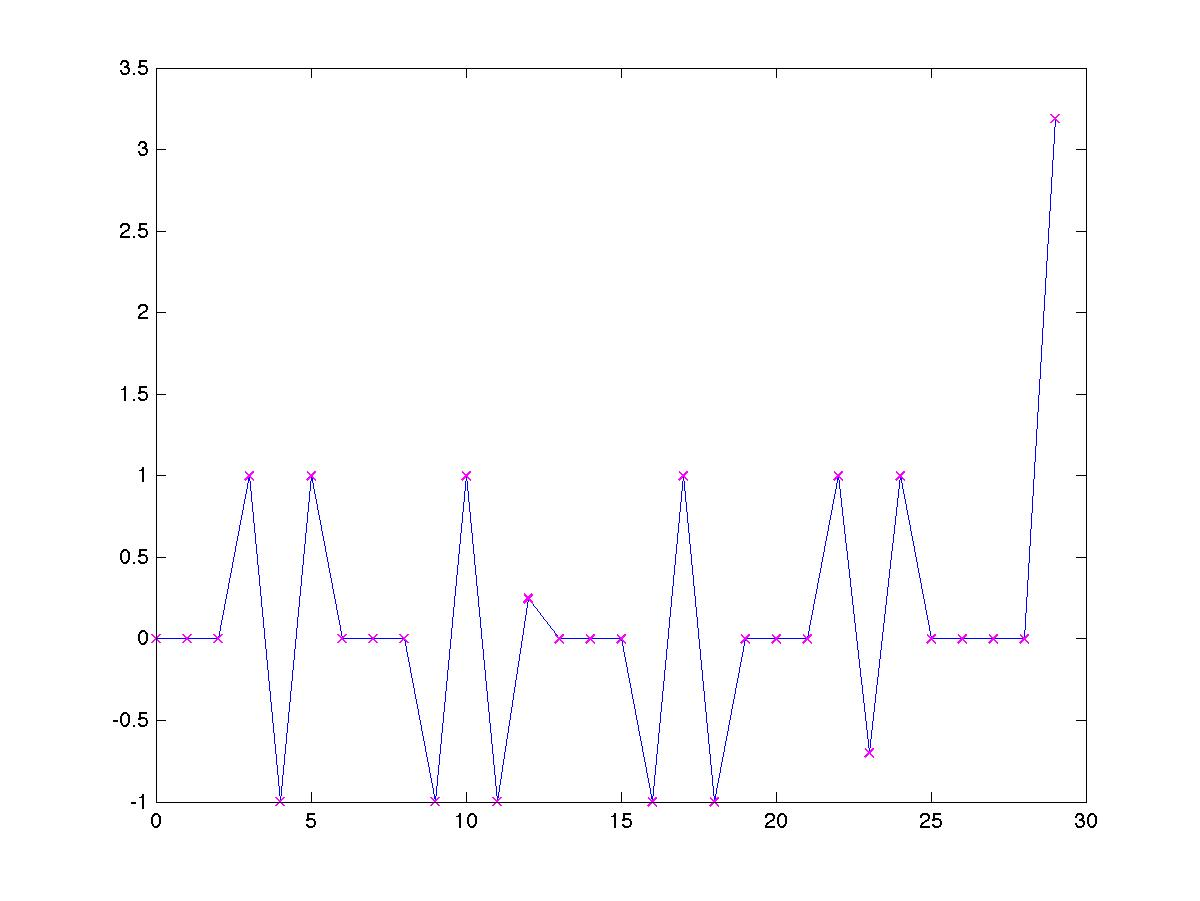
\includegraphics[scale=0.3]{hw3_p317.jpg}
\end{center}
\begin{verbatim}
f=@(x) max(abs(x), 2*abs(x)-1);
F=@(u) sum(f(u));
A = [-1,0.4,0.8;1,0,0;0,1,0];
b = [1;0;0.3];
x_des = [7;2;-6];
N = 30;
KAb = zeros(3,30);
KAb(:,30) = b;
for i=29:-1:1
    KAb(:,i) = A * KAb(:, i+1);
end

cvx_begin
    variable u(N);
    minimize F(u);
    subject to 
        KAb*u == x_des;
cvx_end
plot(0:29,u','-b');

clear u
%% alternative solution (LP)
cvx_begin
    variable u(2*N);
    minimize ones(1,N)*u(N+1:end);
    subject to
        KAb*u(1:N) == x_des;
        u(1:N) <= u(N+1:end);
        -u(1:N) <= u(N+1:end);
        2*u(1:N)-ones(N,1) <= u(N+1:end);
        -2*u(1:N)-ones(N,1) <= u(N+1:end);
cvx_end
hold on
handle = plot(0:29,u(1:N)','mx','LineWidth',1.2);
saveas(handle, 'hw3_p317','jpg');
\end{verbatim}
\end{document}
